% !TEX root = main.tex

\section{Ethereum Trading Graph Analysis}
To exploit information hidden behind the transactions on-chain, we construct an Ethereum trading graph (ETG, for short) and then  methods such as graph embedding could be implemented for node classification task.

In this section, we illustrate our approach at first and then discuss differences to other graphs analysis methods.

\subsection{Methodology}
\label{subsec:methodology}
Our methodology consists of three phases, graph construction, graph embedding and node classification. 

\textbf{Graph construction}
First, all transaction data are collected for graph construction. Generally, we consider the ETG as a directed graph $G=(V,E)$, where node $v \in V$ represents an account and $e \in E$ depicts the edge between two nodes. 

Actually, $V$ is the set of all addresses in Ethereum including both EOAs and SCs, and number of addresses is depicted as $|V|=N$. Note that we use the terms address, account and node interchangeably in the remainder of this paper. $E$ is a set of ordered pairs, where $E=\{(v_i,v_j)|v_i,v_j \in V\}$. The order of an edge indicates the direction of activity (e.g., assets transfer and smart contract invocation) from $v_i$ to $v_j$. %Analogously, the number of edges in ETG is represented as $|E|$.


%In our definition, each edge associates with a weight $w$, which will be discussed later. Hence, $G$ is a weighted directed graph.

\textbf{Graph embedding}
The embedding can be defined as follows: given ETG $G=(V,E)$, we aim to represent each node $v$ in a low-dimensional vector space $\vec{y_v}$. By representing ETG as a set of low dimensional vectors, graph analysis algorithms can then be computed efficiently. 

Typical network embedding techniques such as random-walk based and deep learning based models use the pure network structure to map into the embedding space~\cite{goyal2018capturing}. Our model is primarily motivated as an extension of GCNs (Graph Convolutional Networks), which puts the features of nodes and edges into the representation, since it shows effectiveness for entity classification in large-scale relational data~\cite{kipf2016semi}.

 Generally, a multi-layer Graph Convolutional Network with the following layer-wise propagation rule:

\begin{equation}
H^{(l+1)}=\delta(\tilde{D}^{-\frac{1}{2}}\tilde{A}\tilde{D}^{-\frac{1}{2}}H^{(l)}W^{(l)})
\label{eq1}
\end{equation}

where $H^{(l)}$ is the matrix of activations in the $l$-th layer, and $W^{(l)}$ is a trainable weight matrix in the $l$-th layer. $\delta(\cdot)$ denotes an activation function such as the ReLU$(\cdot)$ = max$(0,\cdot)$. $\tilde{A}=A+I_N$ where $A$ is the adjacency matrix of the graph $G$ and $I_N$ is the identity matrix. $\tilde{D}$ is a diagonal matrix where $\tilde{D}_{ii}=\sum_{j}\tilde{A}_{ij}$.

The method can be understood as special cases of a simple differentiable message-passing framework.

\begin{equation}
h_i^{(l+1)}=\delta(\sum_{j \in N} \frac{1}{c_{i,j}}W^{(l)}h_j^{(l)})
\label{eq:gcn}
\end{equation}

where $h_i^{(l)}$ is the hidden state of node $v_i$ in the $l$-th layer of the neural network. And $c_{ij}$ is a problem-specific normalization constant which can defined in advance such as $c_{i,j}=\sqrt{d_i d_j}$ where $d_i$ is the degree of node $v_i$.

\textbf{Node prediction}
The final objective of our approach is predicting the node identification in ETG, in essence, classifying given node into categories which are shown in TABLE \ref{tab1}.

By given a labeled account set, supervised or semi-supervised methods can be used for entities classification. Here we simply stack GCN layers of the form which is depicted in Eq.\ref{eq:gcn}, with a softmax($\cdot$) activation on the output of the last layer. A cross-function can be the minimizing objective for training. 

\subsection{Challenges}
\label{section:time}
The graph embedding plays a key part in Ethereum trading graph analysis. The approach \cite{kipf2016semi} inspired us outperforms other methods such as deepwalk~\cite{perozzi2014deepwalk} in experiments on citation networks and knowledge graph dataset. 

However, we found that using such GCN model directly achieves poor effect on ETG which has many properties different from traditional networks (such as social media networks and citation graph). It brings the following challenges.


\textbf{Multi-relations} In ETG, edges stand for different activities such as money transfer, contract creation and contract invocation, which can not be measured in a uniform weight model. For example, a weight of assets transfer maybe the ETH amount, however an invocation to smart contract does not have such numerical value. This inspired us to divide the raw ETG into different relation graphs.

%Our work is motivated as an extension of Relational Graph Convolutional Networks (rGCNs), which is proposed to develop an encoder model for edges in the relational graph~\cite{schlichtkrull2018modeling}. They utilize the transformation of adjacency matrices introduced in GCN to process relational graphs. 

%We divide the edge set into four relations, CALLs with ETH, CALLs without ETH, CREATIONs and REWARDs, according to the their transaction type. Note that the ERC-20 token transfers are categorized as CALLs without ETH which includes normal smart contract invocations as well. The reason is that even though ERC-20 token transfer is a kind of assets transfer intrinsically, it exists in the form of a smart contract in ETG.\footnote{Another reason is that even converting some ERC-20 tokens into ETH is available, the exchange-rate fluctuations make the unification meaningless.}

\textbf{Time information} Even in a specific relation graph, there are repeated edges between the same node pairs. This occurs quite naturally since an account may transfer or invoke to another account repeatedly.

Note that these activities are located at different time intervals along the time axis which are characterized by the block height. Intuitively, a simple solution is to merge those edges by weight summation but this will lose time information. 

\textbf{Second-order proximity} The edge weight $A_{ij}$ in adjacency matrix $A$ is generally treated as a measure of similarity between nodes $v_i$ and $v_j$. And the higher the edge weight, the more similar the two nodes are expected to be. Edges weight $A_{ij}$ is called \emph{first-order proximity} between nodes $v_i$ and $v_j$. 

Further, \emph{second-order proximity} compares the neighborhood of two nodes and treat them as similar if they have a similar neighborhood~\cite{goyal2018graph}. In ETG, two nodes are more similar if they have similar connectivity structures instead of they are just connected by an edge with larger weight. \emph{Second-order} describes the local structure better than \emph{first-order}. As shown in Figure \ref{fig:high_order}, nodes $v_a$ and $v_c$ are smart contracts and node $v_b$ is normal user. Obviously, $v_a$ is not adjacent to $v_c$  but they have similar neighbor structure. Embedding models with \emph{first-order proximity} will keep them far apart although they have similar connection structures, while embedding with \emph{second-order proximity} captures this similarity.


\begin{figure}[htbp]
	\centering
	\subfigure[Example of a high-order proximity caption.]{
		\label{fig:high_order}
		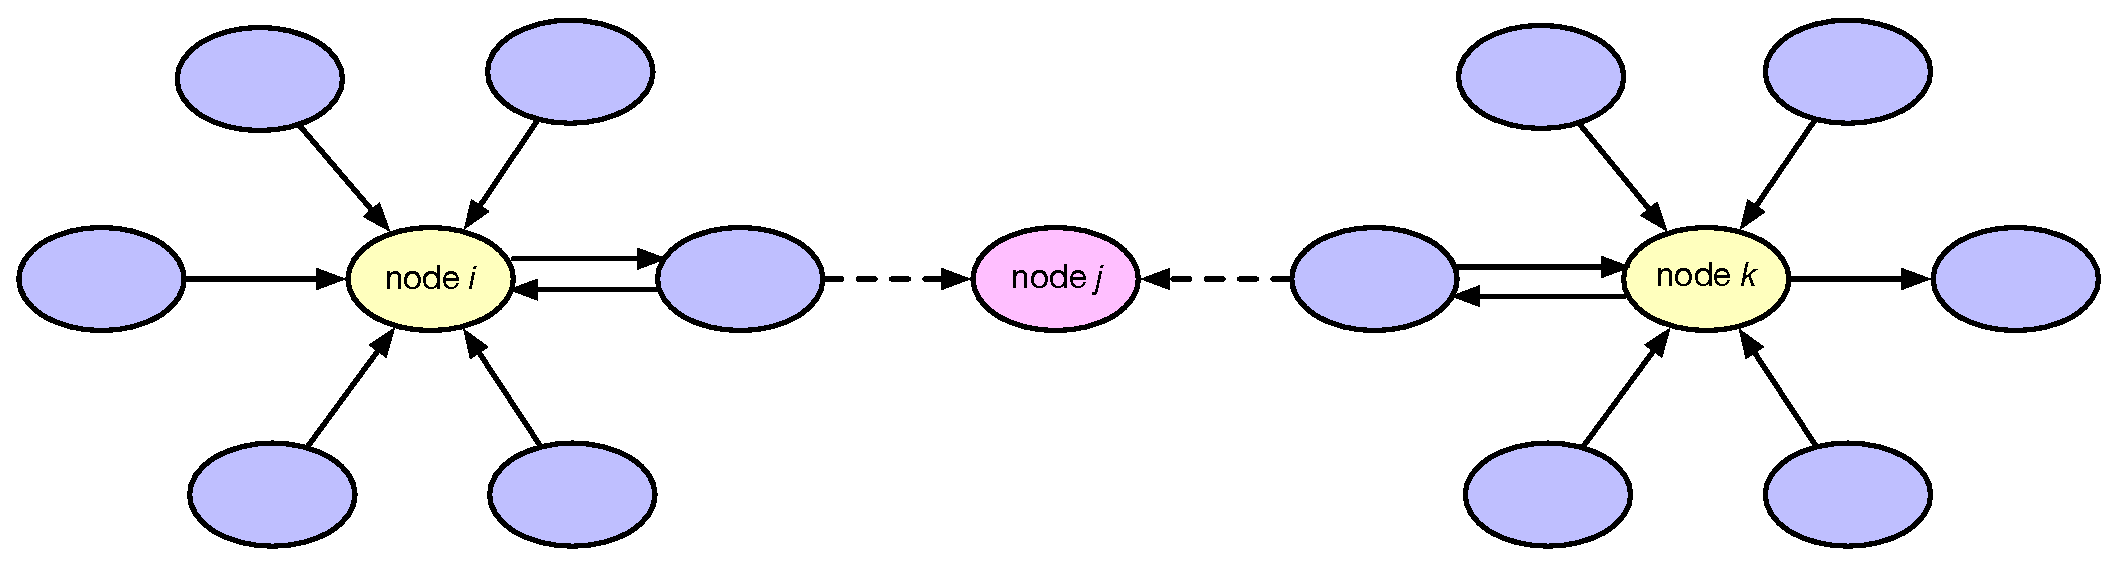
\includegraphics[width=2.0in]{fig/high_order_proximity.eps}
	%\caption{Example of a high-order proximity caption.}
	}
	\subfigure[Example of an asymmetric proximity caption.]{
		\label{fig:asymmetric}
		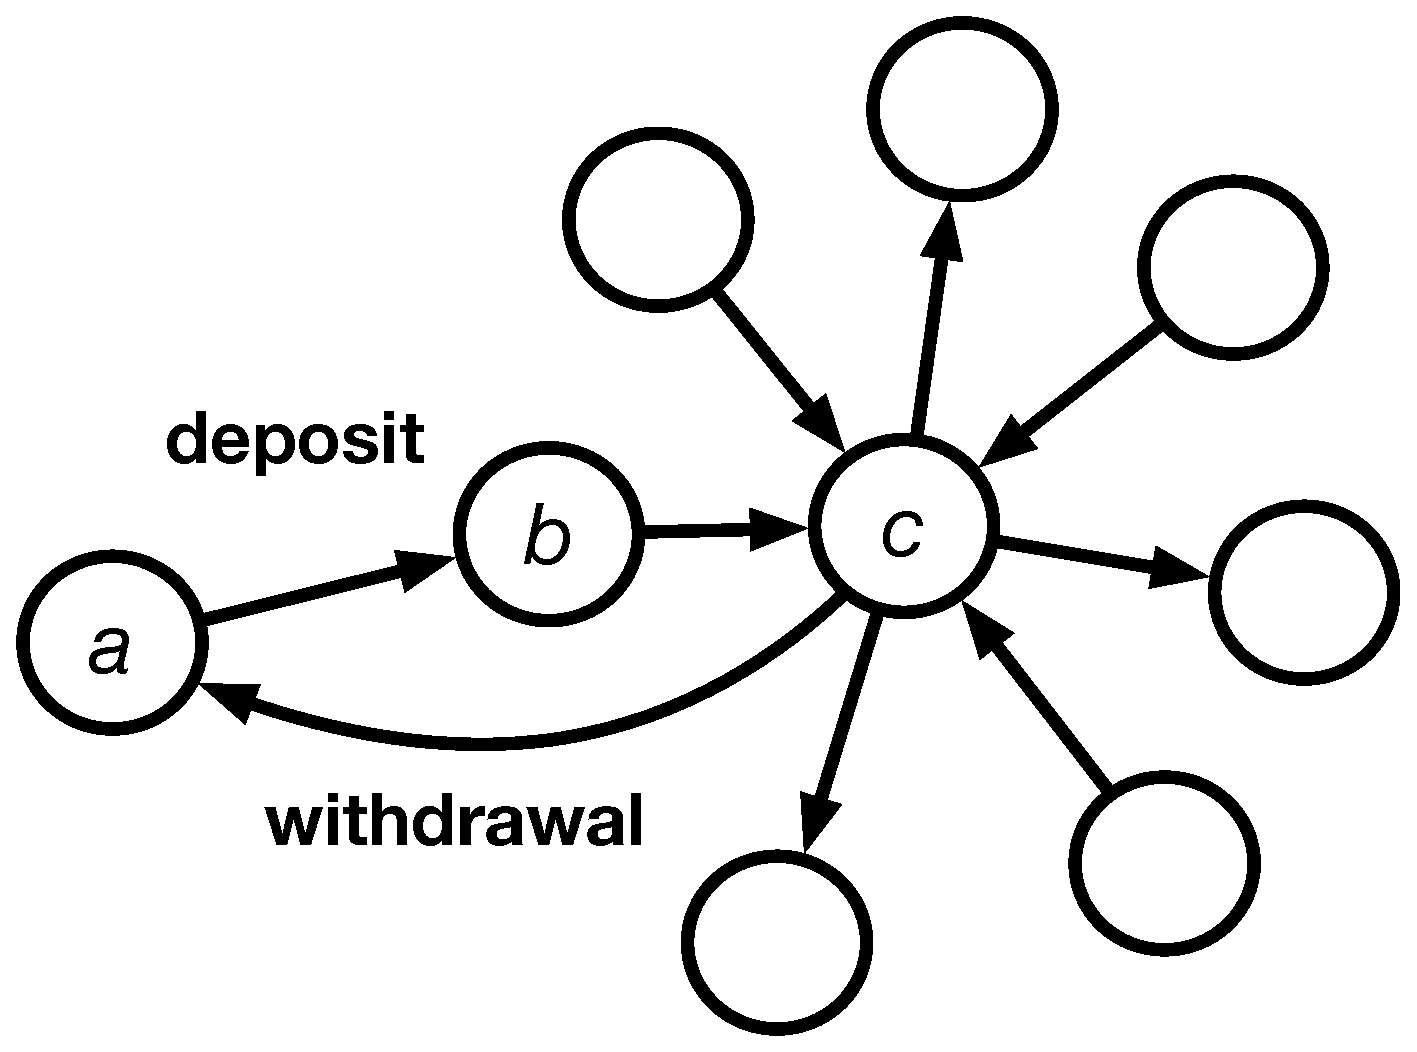
\includegraphics[width=1.5in]{fig/asymmetric.eps}
	}
	\caption{Examples of an asymmetric proximity.}

\end{figure}

%To preserve \emph{second-order} proximity, the hidden layer number in our model is set as 2.
\textbf{Asymmetric proximity}
Another property of closeness in ETG is \emph{asymmetric proximity}. For instance, as shown in Figure. \ref{fig:asymmetric}, node $v_a$ is a Ethereum investor address and node $v_c$ is an exchange root address. Generally, edge weight can be $A_{ab}=A_{bc}=A_{ca}$ since deposit and withdrawal come in pairs in symmetric model. However, the proximity $(v_a,v_c)$ is not equal to proximity $(v_c,v_a)$ due to their asymmetric local structures.

 Zhou et. proposed a scalable asymmetric proximity preserving graph embedding method based on random walk~\cite{zhou2017scalable}. In their model, the probability that $v_a$ arrives at $v_c$ is far less than the one that $v_c$ arrives at $v_a$, as the out degree of $v_c$ is bigger than the out degree of $v_a$. 
However, there is no research on asymmetric proximity in non-probability graph embedding models.

 %due to their asymmetric local structures. However, there is no research on asymmetric proximity in GCN model.
 


%In ETG, two nodes are more similar if they have similar connection structures instead of they are just connected by an edge with larger weight simply or have similar neighborhoods. Using node adjacency as the input, most graph embedding techniques can not preserve such higher order proximity.

%\begin{figure}[htbp]
%	\centering
%	\label{fig_graph_split}
%	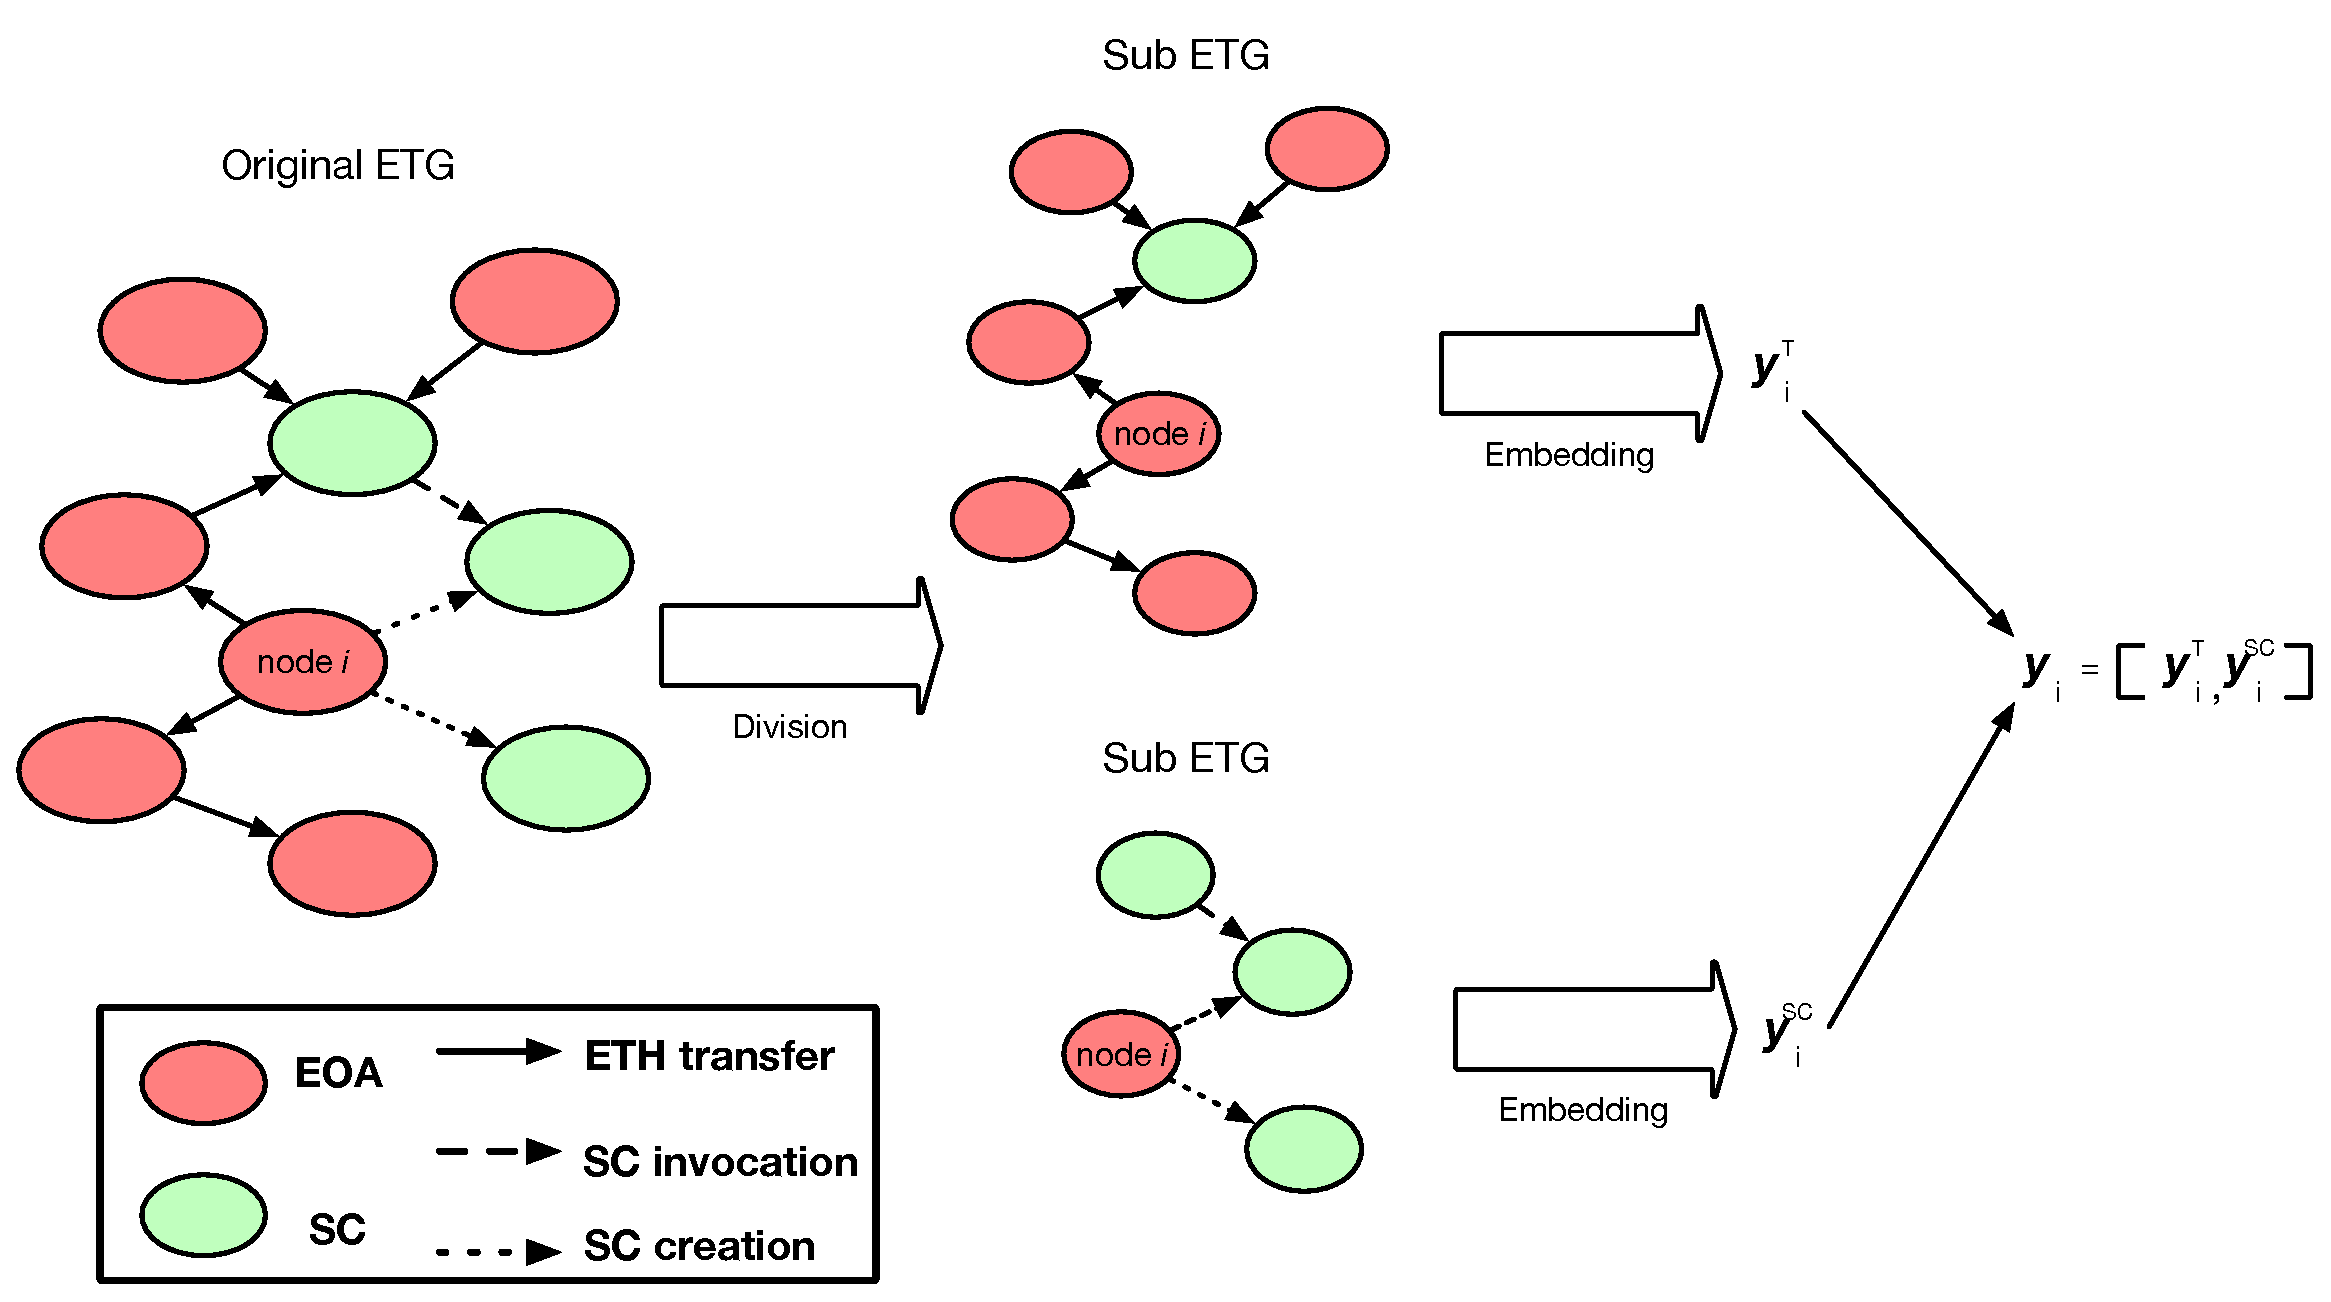
\includegraphics[width=3.5in]{fig/graph_split.eps}
%	\caption{Example of a figure caption.}
%\end{figure}





%Here we introduce a variable named time-density which can be represented as strictly increasing function of block height variance, and the new adjacency matrix in relation $r$ can be represented as 

%\begin{equation}
%\hat{A}=\hat{D}^{-\frac{1}{2}}(\tilde{A}+V)\hat{D}^{-\frac{1}{2}}
%\label{eq:?}
%\end{equation}

%where $V_{ij}$ is the adjacency matrix of time-density from node $v_i$ to $v_j$, and $\hat{D}$ is a diagonal matrix where $\hat{D}_{ii}=\sum_{j}(\tilde{A}_{ij}+V_{ij})$.



